\section{Praktyczne problemy}
W tej sekcji zostaną przedstawione przypadki zastosowania teoretycznej wiedzy wraz z praktycznymi przykładami.



\subsection{Sortowanie wyników}
Czasami zdarza się, że chcemy, aby wyniki zapytania były posortowane według pewnej kolejności. Jest to oczywiście pewien dodatkowy nakład, który serwer MySQL musi wykonać podczas wykonania zapytania. W tym podrozdziale pokażę, co zrobić, aby ta operacja nie wpłyneła drastycznie na wydajność naszego zapytania.

Podstawą optymalizacji sortowania jest używanie indeksów typu B-Tree, co wynika bezpośrednio z faktu, że indeks jest posortowany względem jego kolumn. Aby przedstawić działanie indeksu na realnych przykładach, przygotowałem do tego bazę StackOverflow. Z bazy usunąłem wszystkie indeksy oraz klucze główne założone na wykorzystywanych w przykładach tabelach, aby nie wpływały one na prezentowane przykłady.

MySQL może użyć indeksu do sortowania wyników w następujących przypadkach.



Najlepszym z możliwych scenariuszy wykorzystania indeksu do sortowania danych jest przypadek, kiedy kolumny użyte do sortowania odpowiadają indeksowi, a kolumny, które chcemy zwrócić jako wynik zapytania, są podzbiorem kolumn indeksu.
Weźmy tabelę Users, na którą założymy indeks typu BTREE jak poniżej.

\begin{spverbatim}
	CREATE INDEX Rank_idx ON Users(Reputation, UpVotes);
\end{spverbatim}
Teraz wykonajmy zapytanie:
\begin{spverbatim}
	EXPLAIN SELECT Reputation,UpVotes FROM Users ORDER BY Reputation, UpVotes;
\end{spverbatim}
W takim przypadku poleceni EXPLAIN zwróci w kolumnie EXTRA informację: "Using index", co oznacza, że do sortowania wartości użyty został indeks znajdujący się w kolumnie key, czyli indeks, który przed chwilą stworzyliśmy.

\begin{figure}[H]
	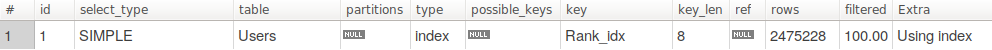
\includegraphics[scale =0.4]{explain15.png} 
\end{figure}
Jeżeli w wyniki chcemy otrzymać jedynie kolumnę \textit{Reputation}, to MySQL wciąż będzie wykorzystywał indeks do sortowania wyników, ponieważ spełnia to warunek zawierania się kolumn rezulatu zapytania w zbiorze kolumn indeksu. Sprawdźmy teraz, co się stanie, jeżeli do klauzuli WHERE dodamy kolejną kolumnę:
\begin{spverbatim}
	EXPLAIN SELECT Id, Reputation, UpVotes FROM Users ORDER BY Reputation, UpVotes;
\end{spverbatim}
\begin{figure}[H]
	
\includegraphics[scale =0.4]{explain16.png} 
\end{figure}
Widzimy, że tym razem MySQL nie wykorzystał indeksu, ale pobrał wszystkie dane i posortował, wykorzystując jeden z dostępnych w MySQL algorytmów sortowania. Co ciekawe, nie zawsze musi się tak stać. MySQL na etapie analizy wykonania sprawdza, czy wydajniejsze będzie dla niego sortowanie wyników na podstawie pobranych danych, czy może, jeżeli sortujemy dane względem jednego z indeksów na tabeli, pobrać ten indeks i wykorzystać do wydajniejszego sortowania. Dodajmy teraz klucz główny dla tabeli Users i sprawdźmy, co się stanie, jeżeli umieścimy go jako jedną z kolumn wyniku naszego zapytania.
\begin{spverbatim}
	ALTER TABLE Users ADD PRIMARY KEY (Id);
	EXPLAIN SELECT Id, Reputation, UpVotes FROM Users ORDER BY Reputation, UpVotes;
\end{spverbatim}

\begin{figure}[H]
	
\includegraphics[scale =0.4]{explain17.png} 
\end{figure}
Wynik polecenia EXPLAIN jest interesujący. Przypomnijmy sobie zatem, w jaki sposób MySQL przechowuje dane w indeksie, jeżeli tabela posiada klucz podstawowy. W takim przypadku wiersze w liściach indeksu są identyfikowane za pomocą wartości kluczy głównych. W naszym przypadku wiersze w indeksie są identyfikowane na podstawie kolumny \textit{id}, co oznacza, że indeks zawiera wszystkie kolumny użyte w zapytaniu.

 Kolejnym często używanym zapytaniem jest pobranie wszystkich kolumn z tabeli, ale sortowanie ich według określonych kolumn. Weźmy następujące zapytanie:
\begin{spverbatim}
	EXPLAIN SELECT u.* FROM Users u ORDER BY u.UpVotes, u.Reputation;
\end{spverbatim}
Tym razem MySQL znów najprawdopodobniej nie użyje indeksu do posortowania danych. Oczywiście nadal może zdecydować, że efektywniejszym będzie dodatkowe pobranie indeksu i wykorzystanie go do sortowania danych.

Przeanalizujmy teraz następne zapytanie.

\begin{spverbatim}
	EXPLAIN SELECT * FROM Users WHERE Reputation = 1 ORDER BY UpVotes;
\end{spverbatim}
\begin{figure}[H]
	
\includegraphics[scale =0.4]{explain18.png} 
\end{figure}
Tym razem MySQL znów wykorzystał indeks, do posortowania wyników. W jaki sposób to zrobił? 
Skorzystał z faktu, że indeksie są posortowane względem kolumn Reputation, a w przypadku, kiedy wartość Reputation jest równa, względem kolumny UpVote, co odpowiada wartości ORDER BY.
Sprawdźmy co się stanie, jeżeli delikatnie zmodyfikujemy zapytanie do postaci:
\begin{spverbatim}
	EXPLAIN SELECT * FROM Users WHERE Reputation > 1000 ORDER BY UpVotes;
\end{spverbatim}

W tym przypadku nie ma jednoznacznej odpowiedzi na pytanie, w jaki sposób MySQL posortuje dane. Optymalizator MySQL musi podjąć decyzję, czy warunki w klauzuli WHERE są wystarczająco selektywne, czy może pobranie indeksu i na jego podstawie przeprowadzenie sortowania będzie efektywniejsze.

\subsection{Przechowywanie wartości NULL czy pustej wartości}
Częstą wątpliwością przy przechowywaniu danych w tabelach MySQL jest pytanie, w jaki sposób reprezentować brak wartości. Załóżmy, że mamy tabelę studentów, która posiada wiersz z numerem domowym studenta. Zdecydowana większość studentów nie posiada numeru domowego. W jaki zatem sposób ustawić wartość w bazie danych. Brak numeru zapisać jako wartość NULL czy może pusty ciąg znaków? Na początku skupmy się na kwestii wykorzystania miejsca na dysku. Przygotowałem cztery następujące tabele:

\begin{spverbatim}
	CREATE TABLE test_null_varchar_values(
	k1 varchar(32) not null, k2 varchar(32) not null,
	k3 varchar(32) not null, k4 varchar(32) not null,
	k5 varchar(32) not null, k6 varchar(32) not null,
	k7 varchar(32) not null, k8 varchar(32) not null);
	
	CREATE TABLE test_not_null_varchar_values(
	k1 varchar(32) not null, k2 varchar(32) not null,
	k3 varchar(32) not null, k4 varchar(32) not null,
	k5 varchar(32) not null, k6 varchar(32) not null,
	k7 varchar(32) not null, k8 varchar(32) not null);
	
	CREATE TABLE test_not_null_int_values(
	k1 int not null, k2 int not null,
	k3 int not null, k4 int not null,
	k5 int not null, k6 int not null,
	k7 int not null, k8 int not null);
	
	CREATE TABLE test__null_int_values(
	k1 int,	k2 int,	k3 int, k4 int,
	k5 int,	k6 int,	k7 int,	k8 int);
	
\end{spverbatim}

Następnie wypełniłem tabele piętnastoma tysiącami wierszy. W przypadku tabeli, które dopuszczają wartość NULL wypełniłem je takimi właśnie wartościami. Dla tabel z kolumnami oznaczonymi jako NOT NULL wypełniłem odpowiednio pustym tekstem ('') lub wartością 0.
Następnie na każdej z tabel wykonałem polecenie ANALYZE TABLE, w celu aktualizacji statystyk i wykonałem polecenie \textit{SHOW TABLE STATUS}, które wyniki umieściłem poniżej na rysunku ~\ref{fig:null_vs_empty_value_analyze_table}.

\begin{figure}
	\caption{Wyniki polecenia ANALYZE TABLE dla tabeli z ośmioma kolumnami}
	\centering
	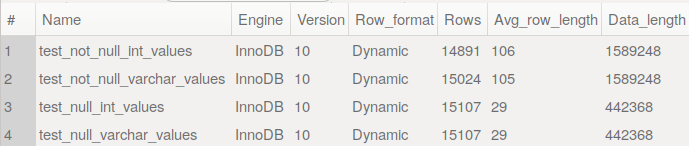
\includegraphics[scale = 0.43]{null_vs_empty_value_analyze_table.png}
	\label{fig:null_vs_empty_value_analyze_table}
\end{figure}

Widzimy, że wykorzystanie NULL zredukować rozmiar danych o ok. 70 \%. Zobaczmy teraz jaki będzie efekt, jeżeli w tabeli będziemy przechowywać tylko jedną kolumnę z możliwymi wartościami NULL. Zmodyfikowałem skrypty tworzące tabele tak, żeby każda tabela posiadała tylko jedną kolumnę. W analogiczny sposób wypełniłem bazę piętnastoma tysiącami wierszy i dla każdej z tabel wykonałem polecenie ANALYZE TABLE. Na rysunku ~\ref{fig:null_vs_empty_value_analyze_table_for_one_column}.

\begin{figure}
	\caption{Wyniki polecenia ANALYZE TABLE dla tabeli z jedną kolumną}
	\centering
	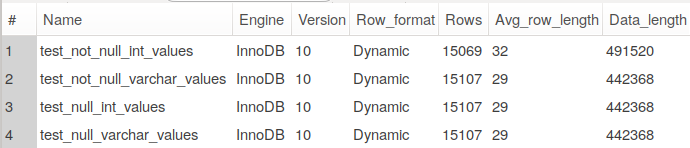
\includegraphics[scale = 0.43]{null_vs_empty_value_analyze_table_for_one_column.png}
	\label{fig:null_vs_empty_value_analyze_table_for_one_column}
\end{figure}

W pierwszej chwili możemy być zaskoczeni jednakowym rozmiarem tabel. Jednakowy rozmiar wierszy zawierających osiem wartości NULL oraz wierszy z jedną wartością NULL wynika ze sposobu w jaki MySQL przechowuje informację o kolumnach z wartościami NULL. Mianowicie, dla każdego wiersza, który zawiera kolumny z wartości przechowywany, jest dodatkowy bajt z informacją o kolumnach z wartością NULL. MySQL na każdym bajcie przechowuje informacje dla maksymalnie 8 kolumn. Gdybyśmy w wierszu zawierającym osiem kolumn, dodali jeszcze jedną z wartością NULL, wtedy MySQL zarezerwowałby dodatkowy bajt dla tego wiersza.


\subsection{Indeks na jednej wielu kolumnach czy wiele indeksów na jednej}
Przed wersją 5.0 MySQL pozwalał na użycie tylko jednego indeksu dla tabeli, nawet jeżeli potencjalnie użytecznych było więcej. W takim przypadku, aby wyszukiwanie na większej liczbie kolumn korzystało z indeksów, należało utworzyć indeks składający się z wilu kolumn. W wersji 5.0 wprowadzony został algorytm łączenia indeksów (\textit{index merge}). Idea łączenia indeksów umożliwia łączenie różnych indeksów na kolumnach użytych w klauzuli WHERE. Niech jako przykład posłuży tabela \textit{Users}. Na początku założę dwa osobne indeksy na kolumny \textit{reputation} oraz \textit{views} i wykonałem analizę zapytania wyszukującego dane z wykorzystaniem obu kolumn.
\begin{spverbatim}
	CREATE INDEX reputation_idx ON Users(reputation);
	CREATE INDEX views_idx ON Users(views);
	EXPLAIN SELECT count(*) FROM Users where reputation = 1 and views = 1;
\end{spverbatim}
\begin{figure}
	\caption{Wyniki polecenia ANALYZE TABLE dla dwóch indeksów}
	\centering
	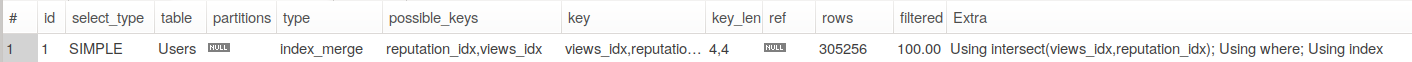
\includegraphics[scale = 0.32]{explain_merge_index.png}
	\label{fig:explain_merge_index}
\end{figure}

Następnie usunąłem zastąpiłem pojedyncze indeksy jednym wielokolumnowym i wykonałem analogiczną analizę.
\begin{spverbatim}
	EXPLAIN SELECT count(*) FROM Users where reputation = 1 and views = 1;
\end{spverbatim}

\begin{figure}
	\caption{Wyniki polecenia ANALYZE TABLE dla pojedyńczego indeksu}
	\centering
	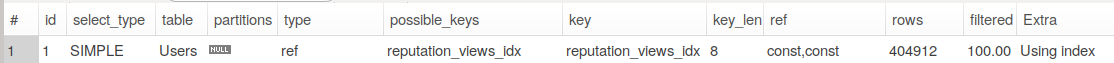
\includegraphics[scale = 0.32]{explain_without_merge_index.png}
	\label{fig:explain_without_merge_index}
\end{figure}

Na rysunkach ~\ref{fig:explain_merge_index} oraz ~\ref{fig:explain_without_merge_index} widzymy wynyniki polcenia EXPLAIN dla obu przypadków. W obu odfiltrowane zostało 100 \% wierszy, więc na pierwszy rzut oka wydaje sie, że pomiędzy tymi dwoma podejściami nie ma znaczącej róznicy. W następnej kolejności zmierzyłem średni czas wykonania obu zapytań. W przypadku pojdeńczego indeksu zapytanie wymagało śrendio 0.05 sekundy, natomiast przy łaczeniu tabel ok. 0.5 sekundy. Na koniec usunąłem indeks dla kolumny \textit{Views}, żeby optymalizator wykorzystał tylko indeks \textit{reputation\textunderscore idx}.
\begin{spverbatim}
	CREATE INDEX reputation_idx ON Users(reputation);
	EXPLAIN SELECT count(*) FROM Users where reputation = 1 and views = 1;
\end{spverbatim}
\begin{figure}
	\caption{Wyniki polecenia ANALYZE TABLE dla indeksu \textit{reputation\textunderscore idx}}
	\centering
	
\includegraphics[scale = 0.32]{explain_with_reputation_idx.png}
	\label{fig:explain_with_reputation_idx}
\end{figure}

Tym razem tylko 10 \% wierszy zostało odfiltrowane, a średni czas wykonania zapytania zbliżył się do 8 sekund. Jak widzimy mechanizm łaczenia tabel nie będzie równie wydajny co pojedyńczy indeks na wielu kolumnach, ale może być dobrą alternatywą do pełnego przeszukania lub wykorzystania jedynie jednego indeksu.
\subsection{Sztuczny czy naturalny klucz główny}
TODO

\subsection{Monitorowanie zapytań - \textit{Slow log}}
TODO

\subsection{Konfiguracja serwera}
TODO, jeżeli starczy czasu

\subsection{Ograniczenia klucza zewnętrznego}
Jako przykład dla tego problemu użyłem tabeli 
